\taskpic{ Вертикально закреплённое кольцо имеет радиус $R$ и толщину
  $h$. В кольцо залита жидкость объёма $V$. Какова частота малых колебаний
  жидкости вокруг положения равновесия?}
{
  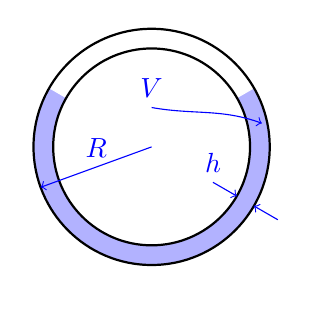
\begin{tikzpicture}
    \draw[fill=blue!30,draw=white] (2,2) ++(30:1.25) -- ++(30:0.25) arc (30:-210:1.5) --
    ++(-30:0.25) arc (-210:30:1.25);
   \draw[thick] (2,2) circle (1.5cm);
   \draw[thick] (2,2) circle (1.25cm);
   \draw[blue,->] (2,2) -- ++(200:1.5cm) node[midway,above] {$R$};
   \draw[blue,->] (2,2)  ++(-30:0.9cm) node[above] {$h$} -- ++(-30:.35cm);
   \draw[blue,->] (2,2) ++(-30:1.85cm) -- ++(-210:.35cm);
   \draw[blue,->] (2,2.5) node[above] {$V$} to[out=-10,in=160] (3.4,2.3);
  \end{tikzpicture}
}